%************************************************
\chapter{Implementation}\label{ch:implementation}
%************************************************
In order to validate the metric,
an application that appealed both to developers as well as employers
needed to be built. It should motivate developers enough to grant it access to their
public repositories, and convince recruiters to use it. The special means that
the development of the application required will be described in this chapter.

\section{Employee view}
registration for ranking
statistics
ranked xth for some request

\section{Employer view}
enter some criteria
receive ranking
ability to look at profiles through this ranking

\section{Architecture}
Web applications are state-of-the art as they require little servicing
and no complex versioning. The use-case of many users taking
advantage of a common dataset was perfect for it.
We decided to implement the serverside logic in NodeJS, which is a
JavaScript runtime. The client-side runs in the browser and makes
use of standard web technologies like CSS3, HTML5 and Javascript.
The analysis results are saved in a SQLITE3 database.
\newline

The serverside part needs to master two tasks: serving data to clients
as well as analyzing repositories from developers.
These are obviously two very different concerns.
In order not to stall one of the tasks while executing the other,
we decided to have two dedicated processes running alongside each other.
One of these will serve the data and perform queries on the database,
while the other will keep the local copies of repositories up to date and run
the metrics on them. We will call the first the \textit{hirebot} and the
latter the \textit{analyzer}.

\subsection{Hirebot}
The component that plays the webserver role is called \textit{hirebot}.
It attends the usual webserver tasks like formatting templates and querying
the database for answering HTTP requests to an endpoint.
\newline

Additionally it implements the foundation for future data analysis.
It allows developers to register with GitHub to grant the application
access to their emails and their repositories. Hirebot then notifies
the analyzer of this additional datasource. The repositories are then cloned
and analyzed. This process is also depicted in figure \ref{fig:regprocess}.

\begin{figure}
  \centering
  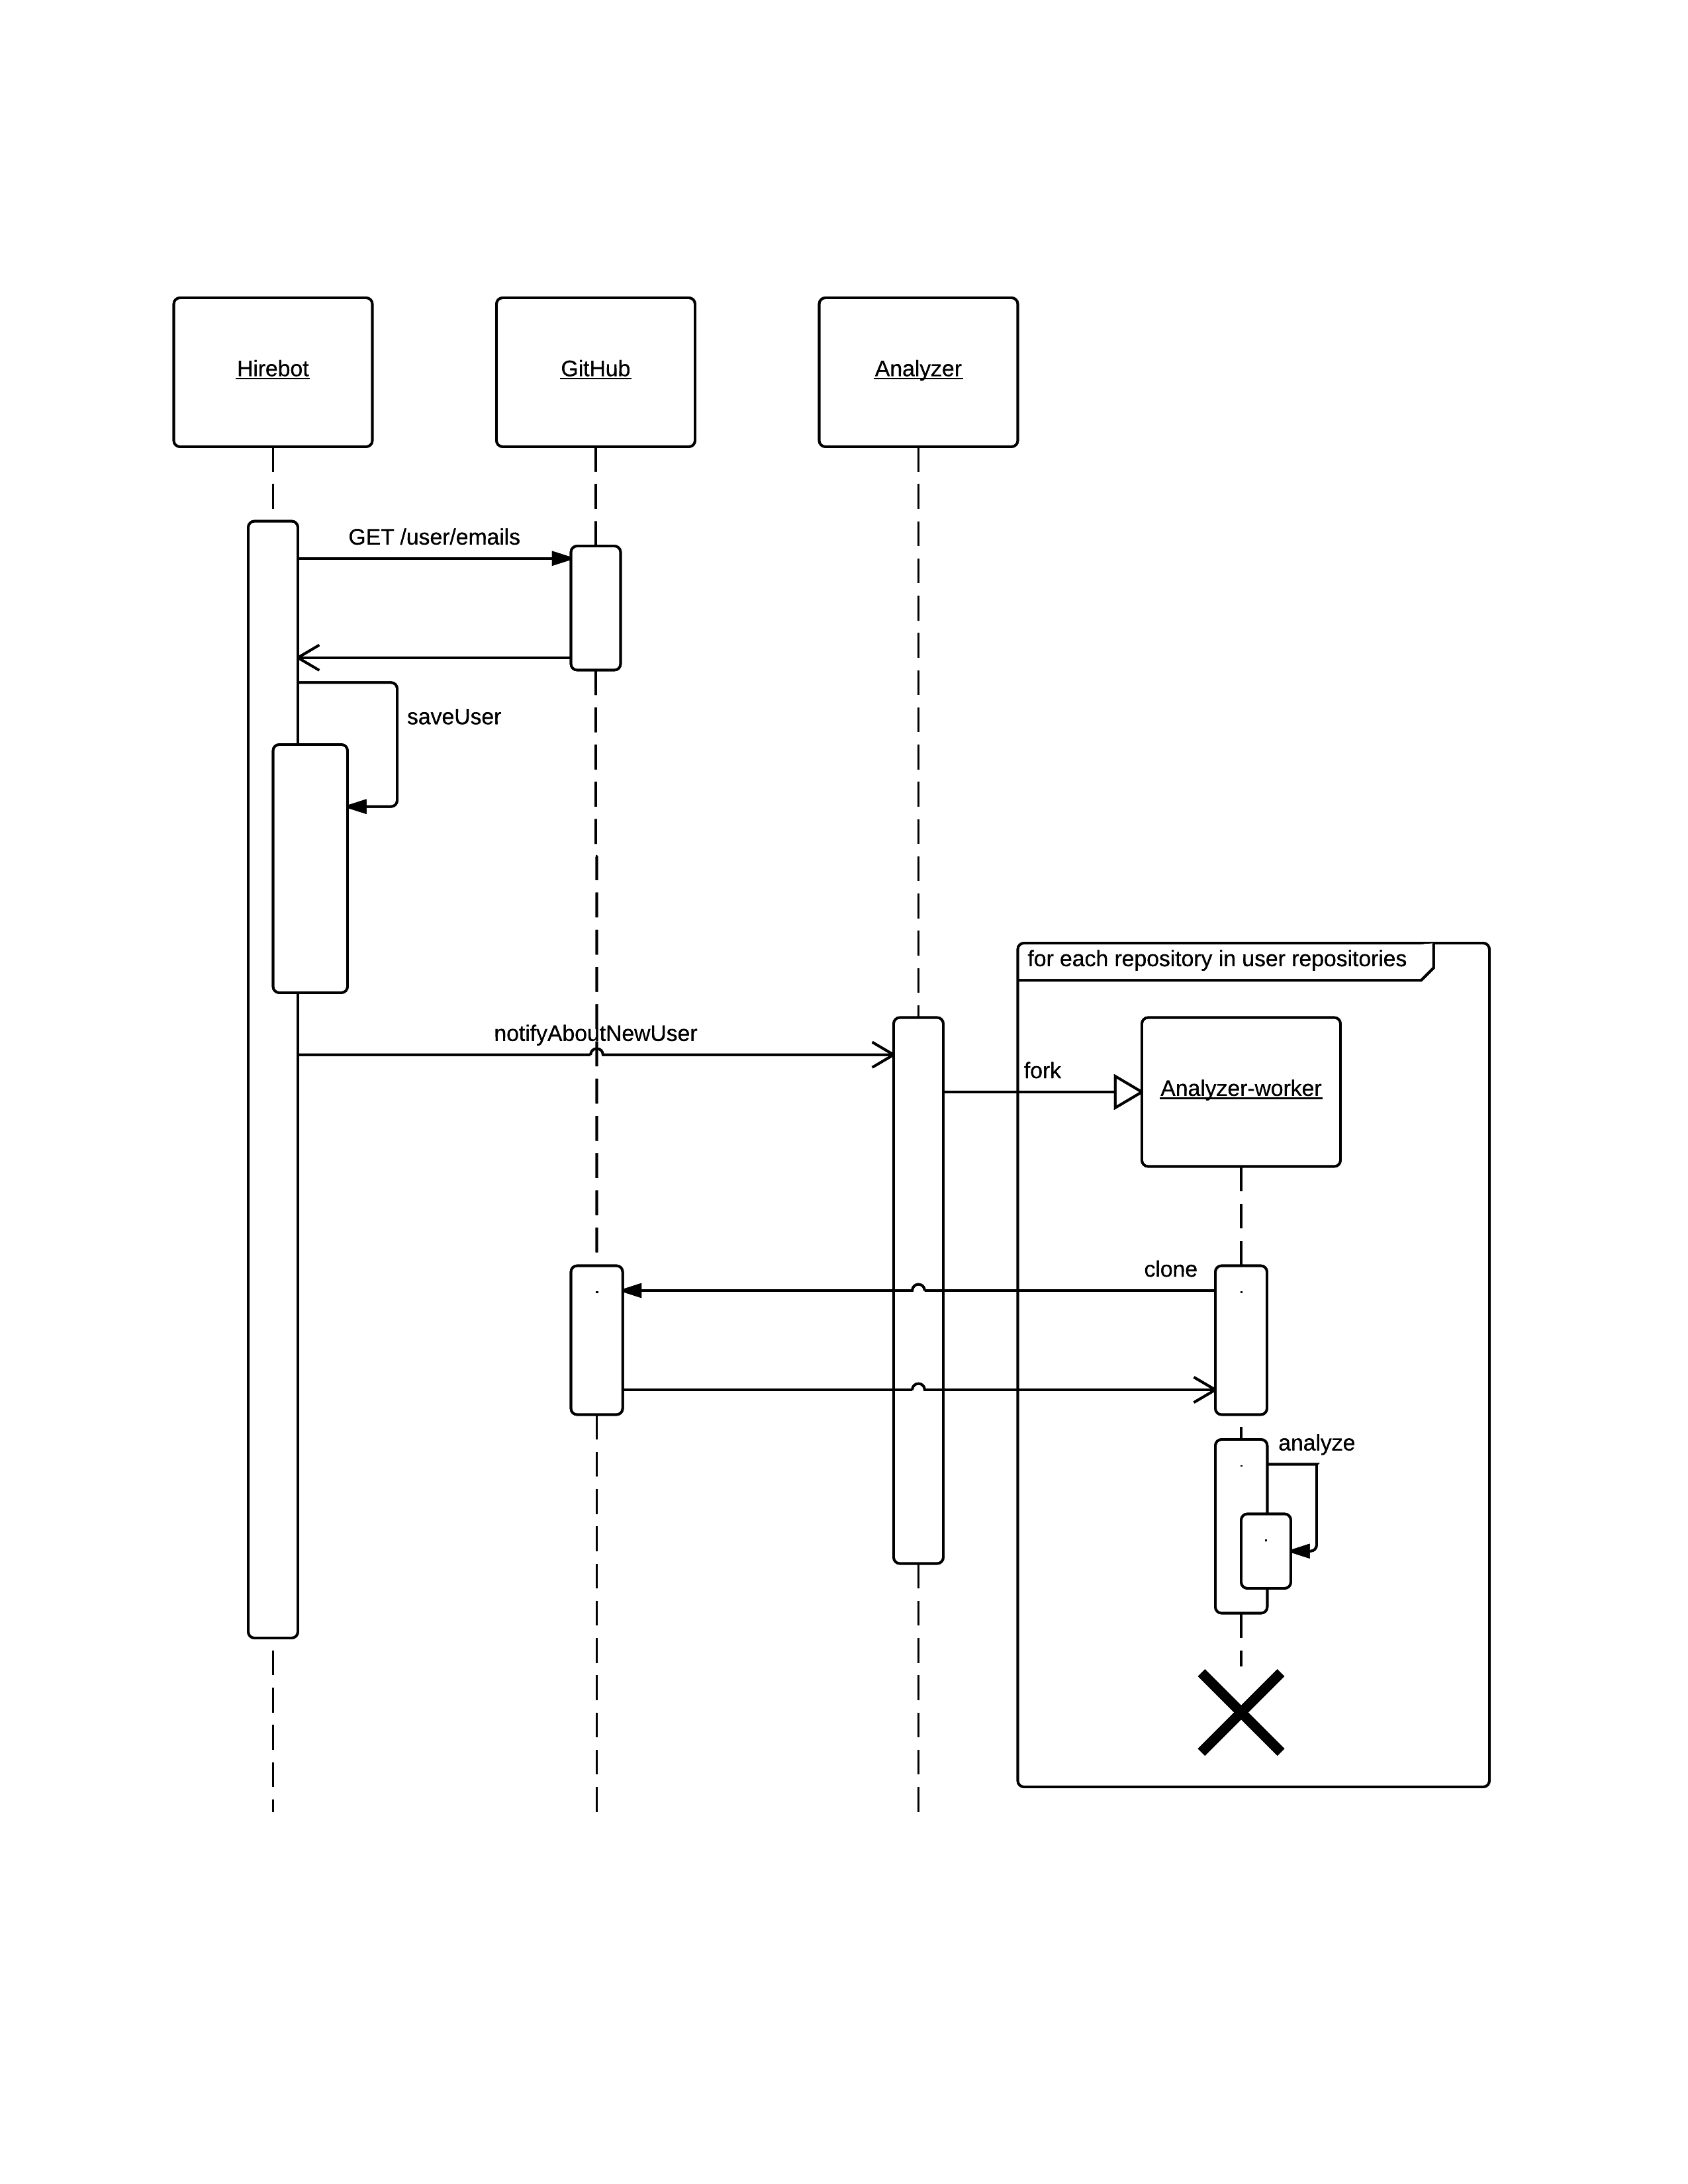
\includegraphics[width=35em]{gfx/registersequence.png}
  \caption{The interplay of the three processes after the OAuth 2.0 dance has been completed.}
  \label{fig:regprocess}
\end{figure}

\subsection{Analyzer}
%TODO rewrite because of restructuring...
The analyzer component of the application handles two slightly different
tasks. First, it has to schedule an initial clone of all repositories
a user owns upon his registration. Then, it has has to keep those local
copies up to date and add new repositories, should there be any.
\newline

These are certainly no impossible tasks, but \textit{nodegit}, the library
that was used for accessing the git repository data, was
leaking memory strongly and to counter this, a sub-process structure was
implemented. The analyzer itself only executes management logic,
schedules the analysis, and communicates with the hirebot process.
For executing the analysis, it forks an \textit{analyzer-worker} for each
single repository. The worker clones or updates that repository,
runs the analysis, saves the results into the database and terminates
upon completion. The forks are done sequentially to avoid putting
too much load on the system at once.

\subsection{Database schema}
The database schema of hirebot is not very complex.
Users are central to the application and every other type of data
is associated with one, as seen in figure \ref{fig:schema}.

\begin{figure}
  \centering
  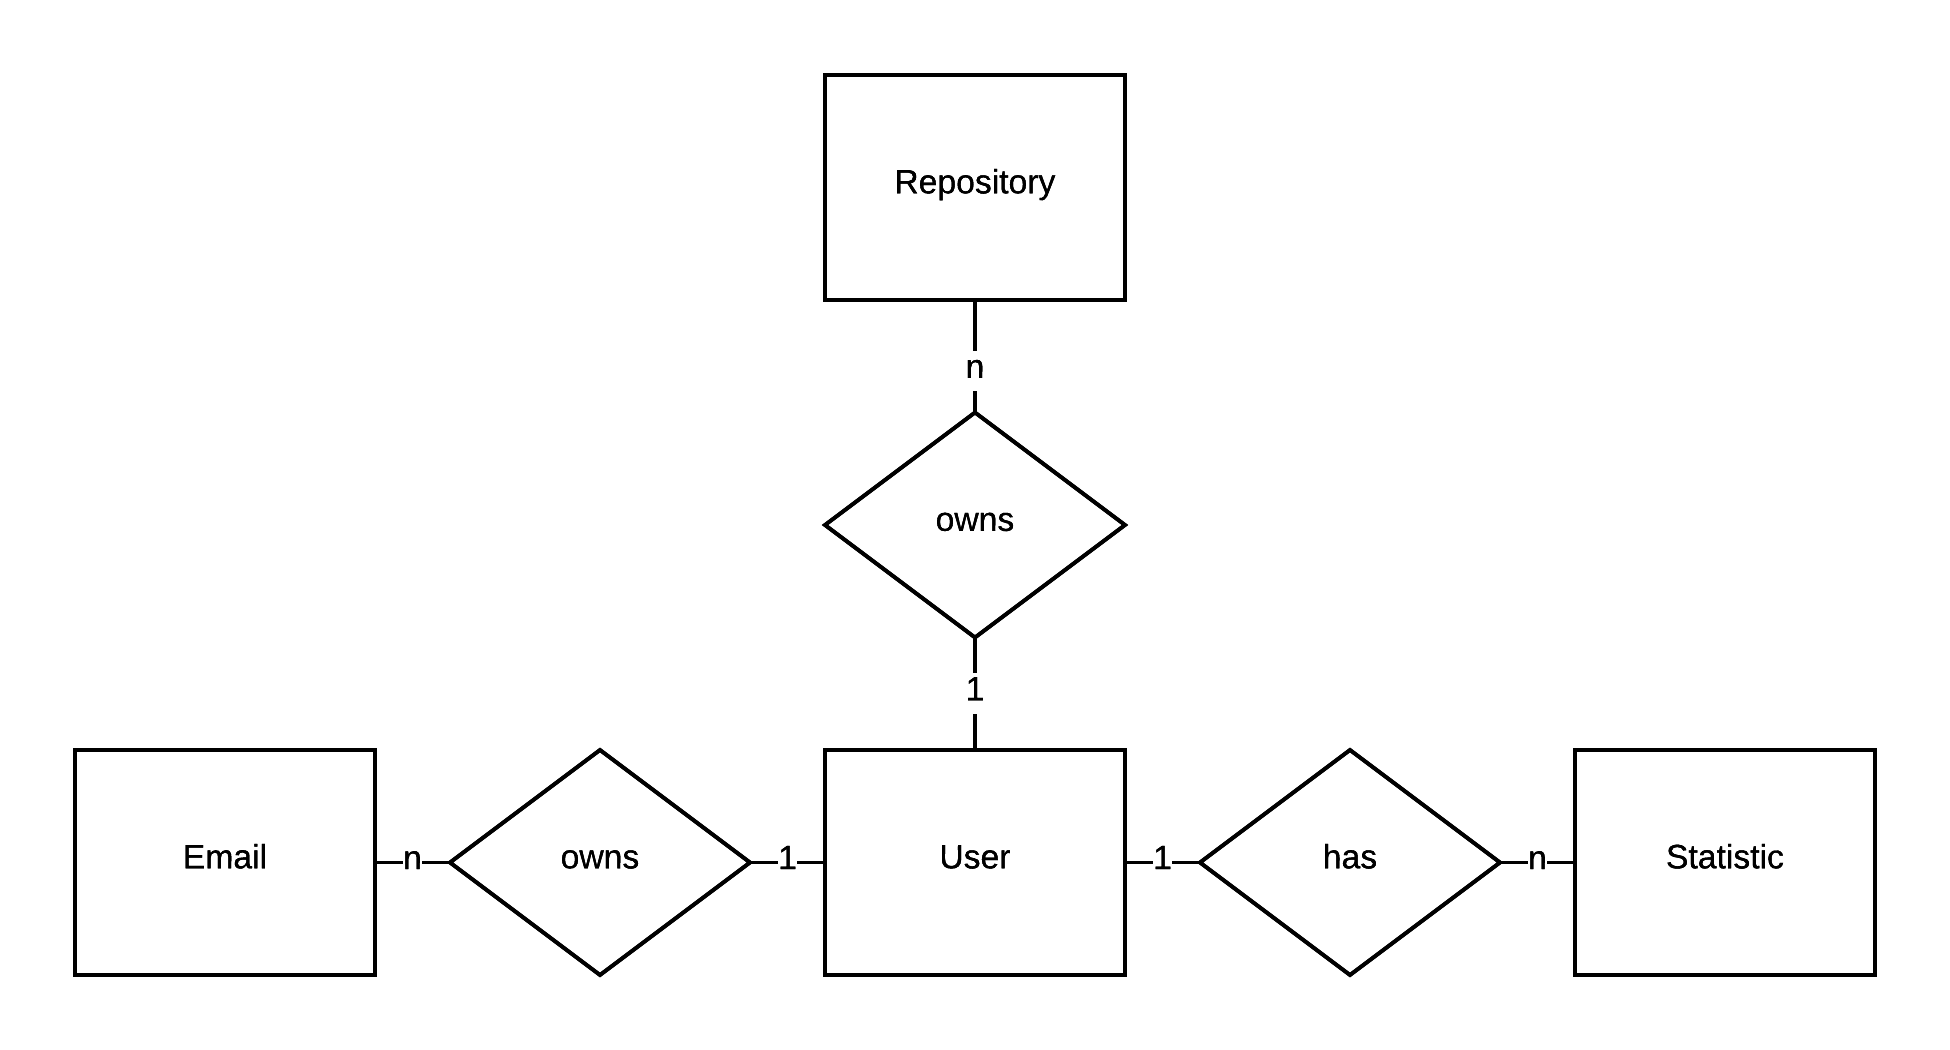
\includegraphics[width=20em]{gfx/schema.png}
  \caption{The hirebot database schema}
  \label{fig:schema}
\end{figure}